\section{Setup}

\section{Single flow overhead}

\textbf{Throughput}

\begin{figure}
    \centering
    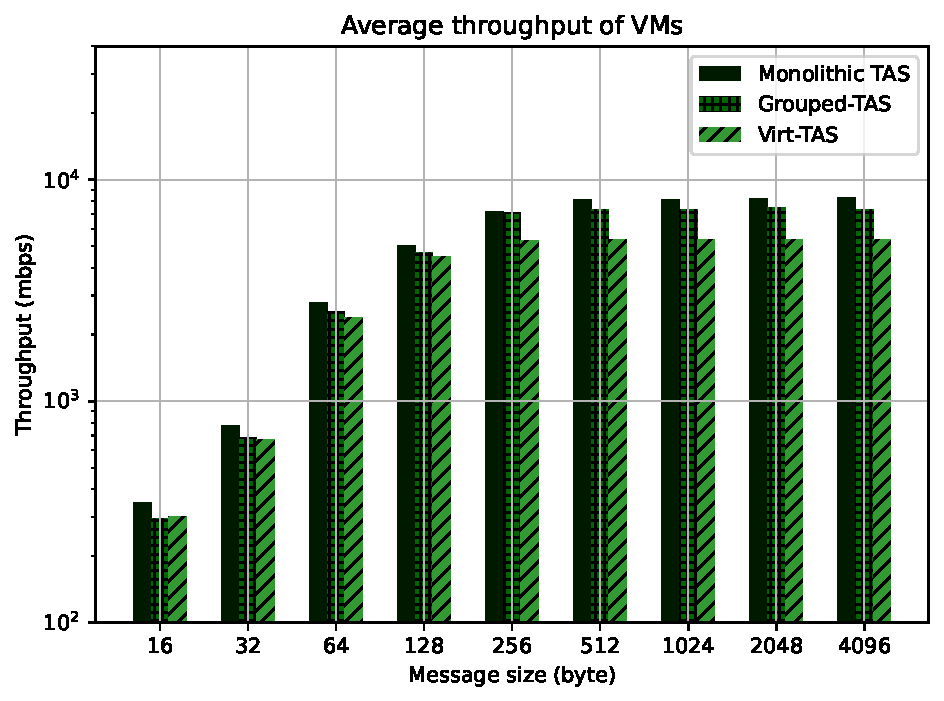
\includegraphics[scale=0.8]{../results/overhead.throughput.pdf}
    \caption{Single context overhead.}
    \label{fig:overhead.throughput}
\end{figure}

\textbf{Latency}





\section{Multiplexing}

The goal of multiplexing experiment is to validate the enhancement of VirtTAS in terms of 
higher throughput and resource efficiency. Specifically, the experiment 
investigates the ability of VirtTAS to benefit from multiplexing of packet processing 
across multiple VMs through a shared TCP fast-path. 

To this end, we conduct three different scenarios, as illustrated in Figure 
\ref{fig:multiplexing.experiment}. In each of the scenarios, we configure four 
VMs across two servers. The servers in this experiment are interconnected directly. 
Subsequently, we execute a Micro-RPC benchmark between these four pairs of VMs, 
with message sizes from 16 to 4096.


In the first scenario (\emph{kernel}), we follow the conventional 
setup where applications running on the VMs utilize the conventional kernel 
networking. In this scenario, the hypervisor establishes connectivity to VMs through 
TAP devices, while a virtual switch applies virtualization policies to the network. 
For the setup, we allocate three cores to each VM, and the server and client applications 
are using three threads to leverage all available cores. 
Additionally, the virtual switch runs on one core. Overall, the scenario employs
a total of 13 cores. 

In the second scenario (\emph{Independent-TAS}), we execute the TCP acceleration service on each VM, 
utilizing two cores for the service and one core for the application itself. 
The goal is to optimize TCP packet processing within the VMs, 
to increase throughput and reduce latency for the applications. 
Similar to the first scenario, the virtual switch applies virtualization policies 
to packets on the hypervisor, and the experiment consumes 13 cores.


In the final scenario (\emph{Virt-TAS}), we deployed VirtTAS on the hypervisor, dedicating four 
cores exclusively to its operations. In this case, each VM is allocated a single 
core for application processing. Notably, this scenario requires only 8 cores,
which is nearly 40\% less cores comparing to previous scenarios.

\begin{figure}
    \centering
    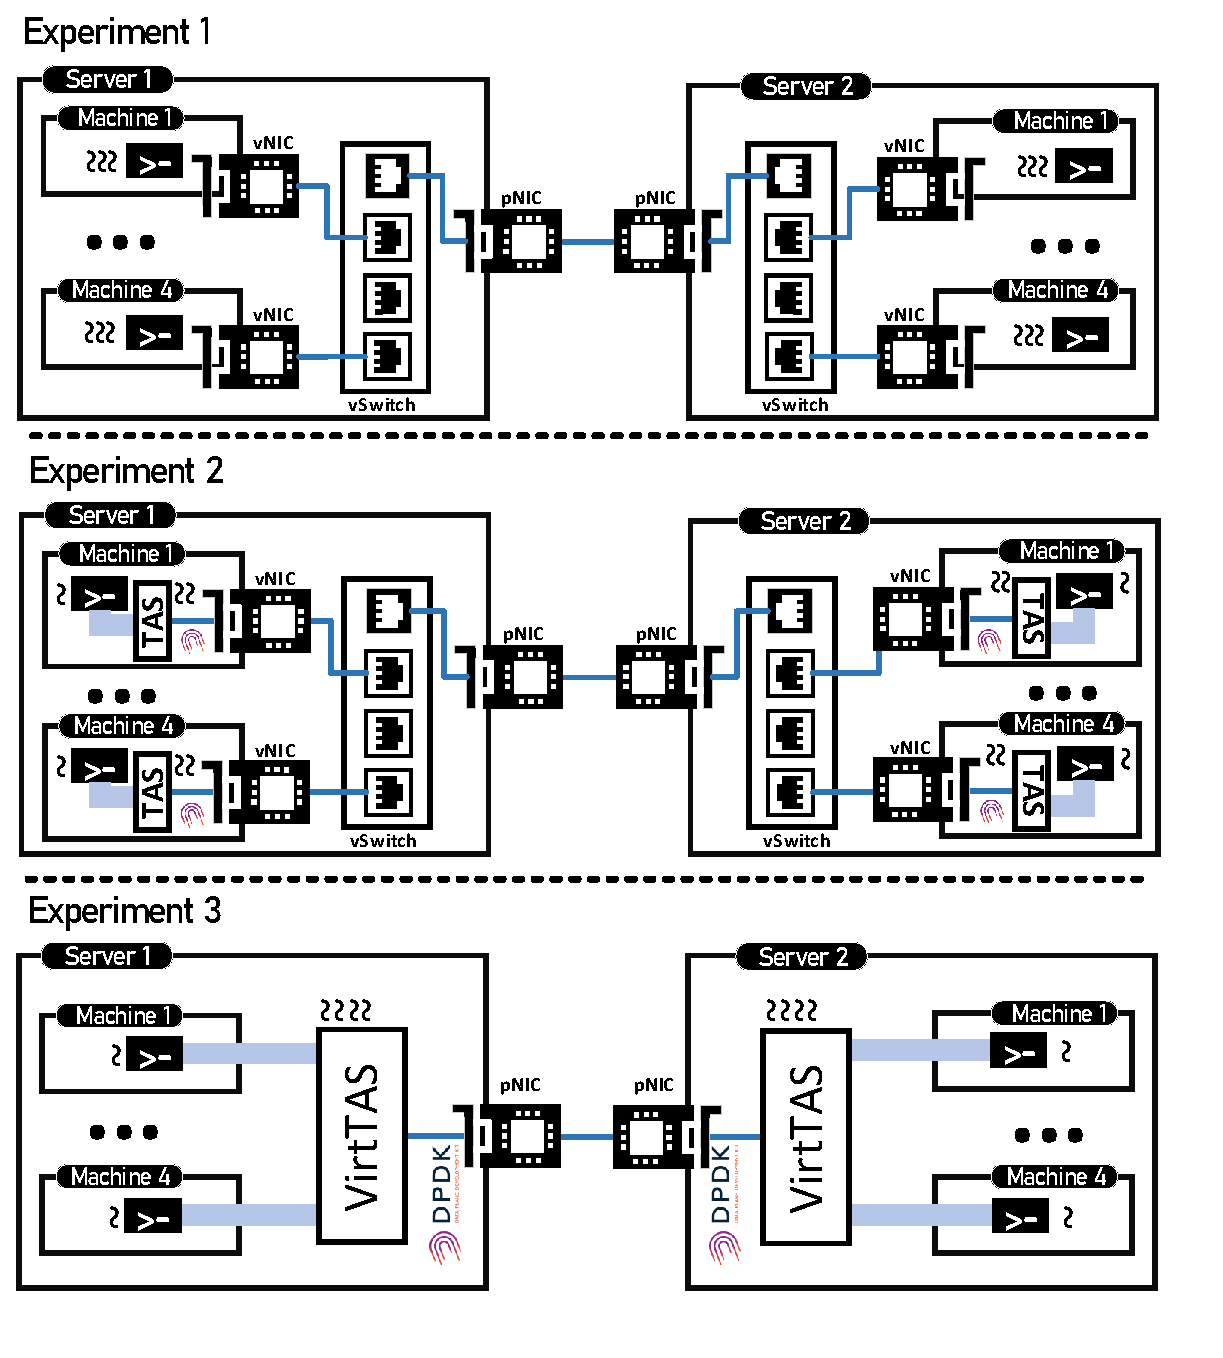
\includegraphics[scale=0.75]{../Figures/multiplexing.experiment.pdf}
    \caption{Multiplexing experiment setup in three different scenarios (\emph{i}) kernel, 
    (\emph{ii}) Independent-TAS, and (\emph{iii}) Virt-TAS.}
    \label{fig:multiplexing.experiment}
\end{figure}

\begin{figure}
    \centering
    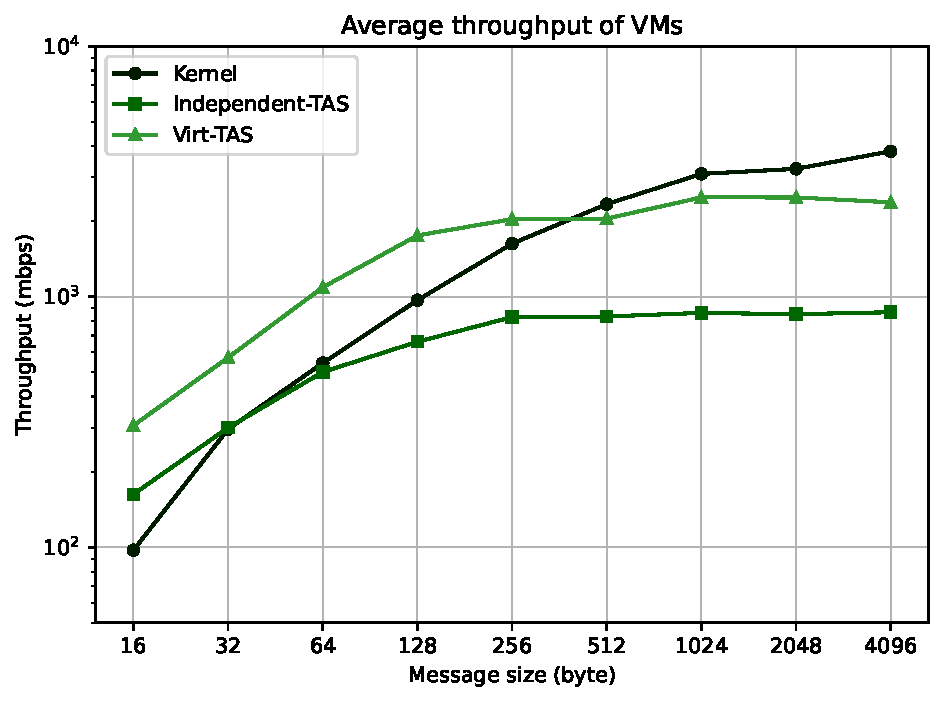
\includegraphics[scale=0.8]{../results/multiplex.throughput.pdf}
    \caption{Throughput of Micro-RPC benchmark in three different scenarios (\emph{i}) kernel, 
    (\emph{ii}) Independent-TAS, and (\emph{iii}) Virt-TAS}
    \label{fig:multiplex.throughput}
\end{figure}
